%% LyX 2.1.4 created this file.  For more info, see http://www.lyx.org/.
%% Do not edit unless you really know what you are doing.
\documentclass{UNCC-thesis}
\usepackage[T1]{fontenc}
\usepackage[latin9]{inputenc}
\setcounter{secnumdepth}{3}
\usepackage{array}
\usepackage{float}
\usepackage{graphicx}
\usepackage{nomencl}
\usepackage{algorithm}
\usepackage{algpseudocode}
\usepackage{xcolor}


\usepackage{pifont}% http://ctan.org/pkg/pifont
\newcommand{\cmark}{\ding{51}}%
\newcommand{\xmark}{\ding{55}}

\newcommand{\dm}[1]{{\color{blue} DM Says: #1}}


% the following is useful when we have the old nomencl.sty package
\providecommand{\printnomenclature}{\printglossary}
\providecommand{\makenomenclature}{\makeglossary}
\makenomenclature

\makeatletter





%%%%%%%%%%%%%%%%%%%%%%%%%%%%%% LyX specific LaTeX commands.
%% Because html converters don't know tabularnewline
\providecommand{\tabularnewline}{\\}

%%%%%%%%%%%%%%%%%%%%%%%%%%%%%% User specified LaTeX commands.
% If you are using MikTeX on Windows and you have a nomenclature section
% you may want to uncomment the line below.
%
%\immediate\write18{makeindex msthesis.nlo -s nomencl.ist -o msthesis.nls}

\graphicspath{ {./figs/} }

\@ifundefined{showcaptionsetup}{}{%
 \PassOptionsToPackage{caption=false}{subfig}}
\usepackage{subfig}
\makeatother

\begin{document}
\pagenumbering{roman}
\fbmatterchapterformat
% Doctype should be either dissertation proposal, dissertation, or thesis.
% If you're getting a master's, specify "thesis" below.
% If you're getting a PhD, specify "dissertation" below.
\doctype{thesis}
%%%%%%%%%%%%%%%%     IMPORTANT! IMPORTANT! IMPORTANT! %%%%%%%%%%%%%%%%
% The rules below MUST be followed for the abstract page and chapter titles
% to be correctly formatted.
%
% 1. Only the first letter of the entire title should be capitalized to allow the
%    title to appear as required by the graduate school on the Abstract page.
% 2. Write chapter titles in ALL CAPS.
%
\title{Risk Aware Motion Planning in Partially Known Environments}
\author{Aryan Gupta}
\degree{Master of Science}
\major{Computer Engineering}
\publicationyear{2023}

\advisor{Dr. Dipankar Maity}

% Add the full name and title of all your committee members,
% apart from your advisor, one by one.  The style file expects
% 3 to 5 committee members in addition to your advisor.

\committeeMember{Dr. Person B}
\committeeMember{Dr. Person C}


% Generate the preliminary title page and copyright page.
\maketitlepage
% \makecopyright
% \begin{abstract}
%     You must have an abstract. The content of your abstract goes here.

%     You should compose the abstract using the conventions of your field. In many fields this section is typically 1-2 pages.
% \end{abstract}

% \begin{dedication}
% If you decide to have a dedication page, your dedication text would
% go here.

% The Dedication page, if used, pays a special tribute to a person(s)
% who has given extraordinary encouragement or support to one's academic
% career.
% \end{dedication}

% \begin{acknowledgements}
% If you decide to have a acknowledgements page, your acknowledgement
% text would go here.

% The Acknowledgement page should be brief, simple, and free of sentimentality
% or trivia. It is customary to recognize the role of the advisor, the
% other members of the advisory committee, and only those organizations
% or individuals who actually aided in the project. Further, you should
% acknowledge any outside source of financial assistance, such as GASP
% grants, contracts, or fellowships.
% \end{acknowledgements}

\tableofcontents{}
% \listoftables
% \listoffigures

\newpage

\renewcommand{\nomname}{LIST OF ABBREVIATIONS}
% uncomment line below to title your nomenclature list as LIST OF SYMBOLS
%\renewcommand{\nomname}{LIST OF SYMBOLS}
%
% NOTE: IF YOU USE A LIST OF ABBREVIATIONS / LIST OF SYMBOLS and are using command-line LaTeX (not LyX)
% YOU MUST COMPILE THE NOMENCLATURE INDEX
% example:
% bash$> pdflatex msthesis.tex
% bash$> makeindex msthesis.nlo -s nomencl.ist -o msthesis.nls
% bash$> pdflatex msthesis.tex
%
\addcontentsline{toc}{chapter}{\nomname}\settowidth{\nomlabelwidth}{ECE}
\printnomenclature{}
\nomenclature{DJK}{Dijkstra's [Algorithm].}

\newpage
\setcounter{page}{1}
\pagenumbering{arabic}
% 2 inch top spacing for new chapters

\bodychapterformat
% \begin{preface}
% If you decide to have an introduction page, your introduction text
% would go here.

% Depending on the discipline or the requirements of the student's advisory
% committee, an Introduction may be included as a preliminary page.
% \end{preface}

\chapter{INTRODUCTION}
    % Motivation for this project (One paragraph high level descriptions)
    Motion planning consists of an autonomous agent (e.g., a robot) traversing a path from a start location to a desired goal location while completing a mission, avoiding the dangers of risk, and obeying the physical constraints of the environment.
    %
    A mission is defined by tasks that the agent must complete; these tasks may be ordered, i.e., one task must be completed before another or may be independent.
    %
    A mission may require tasks to be added or removed while the agent is on the field or in the middle of completing one of the assigned tasks.
    %
    This project started off as a simple implementation of a path-finding and task completion algorithm using a product automata and transformed in to a heuristic approach to path-finding that allows for efficiently, live task switching, in unknown and partially known environments.

    % Proposed tools and solutions
    This project proposes an modular algorithm that expands the product automata approach.
    %
    The proposed algorithm calculates the best path utilizing the surrounding information rather than the information as a whole.
    This allows the algorithm to run more efficiently and removed the necessity of computing information that is not needed in the current iteration or context.
    %
    A multilayered graph is a good analogy to explain the core of the algorithm. The product automata, the old method, flattens out the full graph and creates $M\times N$ vertices. However by utilizing a multi layered graph, the task graph and environment graph is kept sepertly and linked through specific key vertices. In other words the environment is "folded" into each edge of the LTL graph. A full description is explained in Section \ref{}.
    %
    % Subsequently, this algorithm is harnessed for the purpose of simulating an agent's traversal within three distinct environmental contexts, each characterized by a diverse array of task types, denoted herein as `X'. The resultant outcomes are meticulously scrutinized in comparative fashion alongside alternative algorithmic configurations, thereby affording a comprehensive examination of the merits and demerits associated with each approach.

    Furthermore, it is posited that the algorithm's utility can be further extended through the incorporating additional heuristics, these heuristics can be tailored to the specific context the agent may be in. In the context of multi-agent systems, the environment graph can be dynamically updated to encompass the actual physical paths traced by coexisting agents, thereby enhancing the graph with more detailed and contextually relevant metrics.
    %
    Additionally, artificial intelligence (AI) can be introduced to serve the purpose of translating human-readable task descriptions into Linear Temporal Logic (LTL) representations. Another use for an AI system is to replace the actual heuristic itself. By passing the environment thorough a computer vision based AI, the AI system can output a heuristic weight for each task graph edge.
    %
    % Lastly, the current pathplanning is done in 2 dimensions (x, y) and the agents height or distance from the ground is kept constant since the agent is assumed to be a ground robot. This algorithm can be extrapolated to the third dimension. This would require 3D cells and can simulate a drone
    %
    It is important to acknowledge that several of these proposed enhancements remain subjects for the future and not in the scope of this thesis. These extensions are discussed in Section \ref{} and the Conclusion (Section \ref{})
    %

    % Challenges
    When creating the product automata example, many challenges arose. One of the main challenges was the inefficient use of computation. In an environment, much of the environment will not be traversed while completing the mission. This was a challenge to eliminate. To overcome this challenge, this algorithm was created. And while trying to implement partially known / unknown environments it was noted that a heuristic function must be inserted to better predict the trajectory it must take to find the shortest path. Two heuristic functions were designed. A node distance heuristic that calculates the ordering of tasks that leads to the shortest distance to the accepting state and a euclidean distance heuristic that calculates the weight of each task graph edge based off the euclidean distance of two targets. Both of these functions are discussed in greater detail in Section \ref{}.

    \dm{Here is a revised version of the Challenges\\
   Existing methods for ensuring assured autonomy in complex missions require the construction of a product automaton, the size of which grows exponentially with the size of the environment and the complexity of the task \cite{papers/books}.
   %
   This presents a significant scalability issue for real-world deployment. Moreover, these methods rely on the robot having perfect knowledge of the environment and perfect sensing capabilities, which are often impractical in many applications.
   %
   Most importantly, these methods are designed for static missions where task descriptions (or their sequence of completion) remain constant over time.
   %
   Incorporating new tasks (or omitting old ones) necessitates a complete reconstruction of the product automaton, which is impractical for real-time deployment due to the aforementioned scalability issue.

   To overcome these challenges . . .

    }




    % Literature Survey (several paragraphs 50-75 papers)

    % Thesis Contribution (couple paragraphs)
    The main contribution of this project is the introduction of a multilayered heuristic graph search algorithm. This builds on previous work of a product automata, risk aware planning. By using the new method, the algorithm can allow live task switching and partially known environments.

    % My contribution as it pertains to product automata / multilayered graph search
    In the product automata algorithm, a flattened graph is constructed using the task graph and the environment graph. This creates, in a worst scenario, MxN vertices, where M is the number of vertices in the task graph and N is the number of vertices in the environment graph. As the environment scales and/or task increases in complexity, so does the flattened graph. By utilizing a layered graph, no product automata is created holistically, but is created as needed while the agent is traversing through the environment. For example, if the agent has just finished task X and has decided that it needs to complete task Y next it will only use the graph for LTL vertices X-Y and the environment and construct the product automata of XY<cross>Env. The task may have 10 or 500 other tasks and vertices, but since these vertices does not impact the current trajectory, the Cartesian product of those vertices do not need to be computed.

    % My contribution as it pertains to unknown environments / heuristical functions and risk
    When introducing partially known or unknown environment, a challenge arises where no information is known for any of the future nodes of the task graph. Since the environment is unknown or only partially known, an accurate judgement of which edges on the graph is the best is not well known. This issue also arises in the product automata case. My proposed solution for this is to construct a heuristic that summarizes the lower environment graph and uses that as a additional weight for the task graph. The two proposed heuristic is the node distance heuristic that calculates the shortest path from the current node to the accepting state node and uses that as the weight for each node. And a euclidean distance heuristic that calculates the euclidean distance between the two task axioms and uses that the weight for the edges. In addition, in partially known or unknown environment, the risk can be changing or updated each cycle of the algorithm. For example, a warhead shell could have caused a change in the environment that is not currently known to the agent. As the agent nears the site of the shell crater, the agent will update its internal environment map and utilize the new environment map to calculate a new trajectory. Since a full product automata will not have to be created (only the local area is updated in the multilayered graph), the algorithm is more computationally efficient.

    % My contributions as it pertains to live task switching
    Since the algorithm does not need to calculate the product automata, and computes it on the fly, the switching of tasks is very cheap. The tasks can be added, removed, and LIFO'd in various ways. When a new task is added, it is overlaid on top of the multilayered graph and incorporated into the overall structure (but now with more layers). Removal of a layer is the same as removing a task from the mission. A separate structure can be used to LIFO multiple tasks, this can be used as a rudimentary priority queue.

    % The main contribution of this project is the introduction of a multilayered graph search algorithm rather than a
    % - Product automata
    % - Risk aware planning
    % - Parially known / unknown environment

    % my contribution:
    % - multilayerd graph search
    % - heuristic search
    % - partial A*

    % allows for
    % - live task switching
    % - partially known / unknown environment

    % Extensions of this Thesis (paragraph summry of previous section)
    This project takes the literature containing product automata and risk aware planning and the author's contributions of utilizing a multilayered graph search and various heuristic functions to create an algorithm that allows for live task switching and also another feature present in the literature: partially known and unknown environments.

    Other heuristics can be added that can be beneficial in other contexts. In the case of a multi agent system, the heuristic can be updated with the actual physical path for other agents to use (embedding rich metrics into the graph). This can allow agents to communicate the shortest path to other agents and this can be used as a weight in the task graph edges similar to but expanding the euclidean distance heuristic. Artificial Intelligence can be added to convert English worded tasks into LTL tasks. Many of these improvements are left for future work, however, it is to the author's dismay that the current state of AI does not give correct translations of English text to LTL, but since it gives an answer (even though its incorrect some of the time), the structure is there. AI can also replace the heuristic function. By giving the machine learning model the current environment and the start and end locations, it can output a heuristic weight for each task graph edge.

    An agent can embed other rich metrics into the environment. Risk may be very lower dimensional in this project, but higher dimensional risk can be utilized. A computer vision algorithm or AI can embed semantic based risk values that can prompt the algorithm to treat different risk areas differently depending on the context.

    \dm{ Structure the introduction in the following way:
        \begin{itemize}
            \item Motivation for this project (One paragraph high level descriptions)
            \item Challenges (One paragraph describing the major challenges for the project)
            \item Proposed tools and solution method (one paragraph)
            \item A new section titled ``Literature Survey"
            \begin{itemize}
                \item This needs to be several paragraphs.
                \item Described how the challenges identified in the second paragraph have been addressed by other researches. Clearly state what are the shortcomings of their work (i.e., identify the gaps in their research).
                \item At least 50 to 75 papers are to be cited in this section. You do not need to describe each paper individually. You can group papers while describing a common attribute (For example, ``An product automata based approach was considered in [5], [7], [9]-[15]. In particular, [5] introduced the notion of xyz to reduce the size of the product automata to increase computational efficiency. However, despite having xyz, the method is still computationally intensive for real-time deployment and suffers from scalability issues.").
            \end{itemize}
            \item A new Section titled "Thesis Contributions"
            \begin{itemize}
                \item This also needs to be a couple of paragraphs. Each paragraph focusing on a key contribution (applying the same algorithm for three different problems, such as hospital, millitary, etc. does not give you three contributions).
                \item Here you should focus one paragraph on talking about the computational efficiency. Another paragraph on how risk is incorporated
                and addressed. The third paragraph is about how to handle time-varying tasks.
                \item Here is a table that you need to complete (feel free to modify the table)
                \begin{table}[h]
                    \centering
                    \small
                    \begin{tabular}{|c|c|c|c|c|}
                        \hline
                        & {Unknown/Partially }  & Limited & Risk-awareness & Time Varying   \\
                        & Environment & Sensing & &  Tasks \\
                        \hline
                    John Doe et. al \cite{}   & \xmark & \xmark & \xmark & \xmark \\
                    \hline
                    This Thesis & \cmark & \cmark & \cmark & \cmark\\
                    \hline
                    \end{tabular}
                    \caption{Contribution of this thesis}
                    \label{tab:my_label}
                \end{table}
            \end{itemize}
        \end{itemize}
        \item A new section titled "Extensions of this Thesis".
        \begin{itemize}
            \item Summarize the contributions of this thesis in one/two sentences. Then focus on all the new research directions that this thesis opens up. This should one paragraph. However, this needs to be solid.
        \end{itemize}
    }

    % Typically in a path finding algorithm with tasks, the environment is broken into cells and converted into a automaton. The states are the cells the environment is made up of and each cell has a 8 transitions, one going up to the cell above it, one coming down from that cell. Each other direction has two transitions, one going into the current cell and one going out. The task the path finding robot must complete is can be represented by an LTL equation, this equation can be converted into a automaton that defined the valid transitions into the various states the task can exhibit.

    % A typical algorithm would calculate the product of these two automaton and then apply a graph search algorithm to find a path from the start to the end. The complexity of this processes is min m x n, where m is the nodes/cells in the environment, and n is the number of nodes in the LTL equation converted into the automaton. In large environments and large task space. This can introduce many inefficiencies. If a corner of the environment is never traveled to, there is no need to calculate the product in this area. This argument can also be used to reduce the number of nodes in the LTL automaton to reduce the complexity. By creating an algorithm that calculates the product automaton on the fly, many of these inefficiencies can be eliminated by a marginal drop in performance (performance being the absolute shortest path from start to finish). This balance between speed and performance is a long standing question that has been puzzling many academic. In this paper, we will see that for small environment and small task space, a conventional product automaton may be beneficial, but for large environments this may offer many benefits such as, partially known environments, unknown environments, risky environments, changing tasks, multi-agent systems and more.


% INTRODUCTION


\chapter{PRELIMINARIES}
    % See https://ora.ox.ac.uk/objects/uuid:41462553-119f-4d35-bf12-7753d50ac05f/download_file?safe_filename=Barbosa_et_al_2022_risk_aware_motion.pdf&file_format=pdf&type_of_work=Conference+item
    % \section{Hardware}
    % The code was run on a AMD Ryzen 9 56XX processor with a XXXX GPU.

    \section{LTL}
        To construct a task the agent must complete, we utilize Linear Temporal Logic (LTL). LTL is an extension to propositional logic with additional modalities referring to time and ordering of propositions. LTL is built from a set of atomic propositions, logic operators, and the LTL temporal operators. Formally, the formula of LTL follows the following grammar:

        \begin{math}
        \phi ::= \alpha | \phi_1 \wedge \phi_2 | \phi_1 \vee \phi_2 | \neg \phi | G \phi | F \phi | X \phi | \phi_1 U \phi_2
        \end{math}

        where $\alpha$ is an atomic proposition and $\phi$, $\phi_1$, and $\phi_2$ are LTL formulas, $\neg$ (negation), $\wedge$ (conjunction), and $\vee$ (disjunction) are logical operators, and $G$ (globally), $F$ (eventually), $X$ (next) and $U$ (until) are temporal operators (Baier et al., 2008).
    % LTL

    \section{Buchii Automata}
        A LTL formula can be converted into a b\"{u}chi automaton.
        For example, a basic LTL example: $Fz \& (!z U c) \& (!z U b)$, where $b$, $c$, and $z$ are atomic propositions leads to a automaton as seen in Figure \ref{ltl-automaton}.
        Since we know that each cell can only contain a single axiom, this automaton can then be pruned to a graph as seen in Figure \ref{ltl-automaton-pruned}.
        This gives us 2 potential ordering of events: $ABCZ$ and $ACBZ$, also represented by the states: $2310$ and $2410$. The algorithm must now create a heuristic map of this LTL graph, which is an exercise further explored in our experiments. Two heuristics are considered in this paper, a basic graph search heuristic and a euclidean distance heuristic. Other heuristics can be considered as an exercise for future work.

        \begin{figure}[h]
        \includegraphics[width=\textwidth]{ltl-automaton}
        \centering
        \end{figure}

        \begin{figure}[h]
        \includegraphics[width=\textwidth]{ltl-automaton-pruned}
        \centering
        \end{figure}
    % Buchii Automata

    \section{Graph Theory}
        Graph theory is the study of graphs, a mathematical construct consisting of interconnected nodes. Each node or vertices are connected to each other via edges, these edges can be bidirectional and/or have a cost or transitional requirement. Graph theory is heavily used in path finding because many abstract concepts can be simplified into a graph and many common algorithms in the study can be utilized.

        Two common algorithm used in this paper is Dijkstra's (Djk) and its sister algorithm A*. both these algorithms can be used to find the shortest path between two nodes in a graph.

        In Djk's all nodes are marked as not visted and set to have infinite distance from the starting node. As nodes are traversed to, its distance is updated and marked as visited. The current node's neighbors are added to a priority queue based off distances from the starting node. A new node is popped off the queue and algorithm is repeated until the target node is reached. By following the min distance, a path from the target node back to the starting node can be extracted. A* is very similar to Djk's but it uses a heuristic function to sort the queue. In the case of this paper, the node with the shortest euclidean distance to the target node is given higher priority. This incentives nodes that are closer to the target node, rather than nodes that are farthest away from the start node.

        Other rich metrics can be attached to both the vertices and edges of the graph and can be used to create a more efficient path finding algorithm. These metrics are discussed later in this paper.
    % Graph Theory

    \section{Product Automata}
        The typical algorithm for a LTL based path finding is to convert the LTL into an automaton. The environment is split into cells and converted into a graph. Each cell has 8 edges. 4 for each cardinal direction out of the cell and 4 more for directions into the cell. Both of these objects are graphs so a product of these two can create a larger graph with all the potential states and transitions. A Dijkstra's algorithm can be used on this larger graph to find the path through the environment while completing the LTL task.
    % Product Automata

% PRELIMINARIES


\chapter{ALGORITHM}
    The explain the algorithm, its subcomponents have been titled below. Each component is explained separately and then combined in Section \ref{}

    \section{Product Automata}
        In the customary approach to this problem is the product automata approach. In this algorithm, the Cartesian product of the task graph is taken with the environment graph and Dijkstra's applied. Code block \ref{} gives an high level algorithm that exemplifies this. Taking the Cartesian product of two graphs involves combining their vertices and establishing connections between pairs of vertices based on specific rules. To do this, you take the vertices from the first graph, let's call it GG, and the vertices from the second graph, HH. The vertices of the Cartesian product G×H are pairs, where the first component is from GG and the second component is from HH. Edges are then created between pairs of vertices in G×H following these rules: two vertices (uG,uH)(uG​,uH​) and \(v_G​,v_H​\) are connected if either uG=vG​ and there is an edge between uHuH​ and vHvH​ in HH, or uH=vH and there is an edge between uGuG​ and vG​ in GG. This process combines the connectivity information from both original graphs, resulting in a new graph where vertices are pairs and edges are determined by the connections in the original graphs.
    % Product Automata

    \section{Environment Processing and Risk}
        An environment is defined by an area with three subareas: risk areas, traversable areas (no risk), and LTL targets. The environment is encoded in an image for easy processing with an computer vision library (i.e. OpenCV). Since an image contains 3 channels: red, green, blue, the channels can be used to encode different parts of the information. The saturation of the channel can also be used to encode information. The channel bounds are from 0 to 255 in an 8bit image. A high saturation value is 255 and a low saturation value is 0. These two axis of information, color channel and saturation together create the environment.
        %
        The risk areas is encoded by the green channel. Areas with high risk is colored with a high saturated green color. Since the image is an 8bit RGB picture. A green value of 255 is the max risk possible. The second area is encoded by the color black. Since there is no black channel, this is an abstract channel defined by RGB values of (0, 0, 0). These areas are traversable and has a risk value of 0 (since the G value is 0). An environment can have only "all-or-nothing" risk or variable risk. This dicotomy is dicussed in commng paragraph.
        %
        The last area is the target area and it is colored red. These areas are also traversable but on overlap with the agent, it can satisfy an LTL condition. Each red target area has its own atomic proposition in the LTL task formula. The color value (0-255) of the red channel encode which atomic proposition it satisfies. Table \ref{} lists some of the possible values that the red channel can take and their respective meaning. The values are chosen arbitrarily and can be adjusted to accommodate more propositions.
        %
        An example of the environment is shown in Fig. \ref{}. This example shows a hospital floor. The room are surrounded by walls (saturated green lines). And the various shades of red are the different rooms. Each red rectangle in the rooms has an LTL proposition attached to them. In this example, there is no variable risk. There either is risk (green) or no risk (black). The risk channel can be further processed with a Gaussian blur to create a risk gradient around the high risk areas in the case other styles of environments.
        %
        In some environments, the risk is more variable. Fig. \ref{} shows an example of a XXXXX. Each green blob has a guassian outline that tapers out the risk into the traversable areas of the environment. This allows the agen to hig the obstacles closer in case the mission requires a high risk but fast path (characterized by a short path length).

        % COMMENT (for comment folding)
                    % \section{Risk Aware Planning}
            %     Various forms of risk are presented to the agent. The first type is the all-or-nothing type of risk. This type of risk will cause the agent to fail the task. This type of risk is represented by a 255 value in the environment and can be seen as the walls and boundary of the environment in Figure \ref{}. The next type of risk is variable risk, and is represented by the values 0-254 in the environment. These can represent various things in the environment such as a liquid spill, loose ground, or quicksand. These risks can change live in the environment and the agent must be able to replan a path through the risk if its worth the shorter path or plan an alternate plan if the risk is deemed too dangerous. The third type of risk is assumed risk or unknown risk. In many cases the risk is unknown or only partially known, in this case the agent must use its best judgement to recalculate a path as new information is uncovered. The risk is concealed using a blurring to simulate a partially known environment or can be omitted entirely to simulate a totally unknown environment, however in this case, the targets must be still given so the agent knows the direction it must travel to compleate the task.

            %     [pk environment](/figs/env2.bmp)

            %     As the agent moves about the environment uncovering the actual risk value and updating the path it should take.


            %     The proposed solution to this problem follows the basic structure seen an Algorithm~1.
            %     The algorithm is broken down into two separate but intertwined path-finding algorithms.

            %     The first layer of pathfinding is on the LTL task. Once the LTL formula is converted into a graph, a preprocesser can assign different weights to the LTL task automata. three methods have been proposed in this paper and is compared to the product automata

            %     - DJK's node distance
            %     - euclidean distance
            %     - prelim path distance

            %     future work
            %     - AI conv network based path distance
            %     - Environment Rich Metrics

            %     In the DJK's node distance heuristic, djikstra's algorithm is run on the graph to determine each node's distance to the accepting state. This is used as a heuristic to determine which path in the LTL task automata to take. However this poses a few problems.

            %     *INSERT DOUBLE BACK PROBLEM HERE*

            %     In order to resolve this issue, an euclidean distance heuristic can be used. a BFS is run on the LTL graph to determine space of all the potential paths that can be taken. Each path is ranked by using the total euclidean distance that path takes. As the agent moves around, the ranking can be used to determine which LTL targets to consider next.

            %     The main issue which this heuristic is that it does not consider the risk involved in each LTL path jump. Two LTL targets could be very close to each other physically (as calculated by the euclidean distnace equation), but a large object could be in the way between the target and another shorter path could be missed. To resolve this, one last heuristic can be considered

            %     prelim path distance. At each @TODO

            %     Since we know which target will lead us to which state, we can use the euclidean distance from each cell to prevent double-backing of our agent
            % % Risk Aware Planning
        % COMMENT

        Finally, the environment can be split into cells in order to convert the environment into a discrete cellified map. The cell size in this example is 8x8 pixels which is a balance between performance and needed accuracy. This value can be adjusted to sacrifice performance in favor of accuracy and granularity. Each cell is given a letter depending on the cell color using the aforementioned area types. Some of these cells are labeled in the image. The "$C$" target is split into cells, Empty cells are labeled by a "$\#$", Hazard cells are labeled by an "$X$", and the actual $C$ target is labeled by a "$C$". Figure \ref{} shows the cell map, the "$\#$" (empty cells) characters are replaced by spaces to show a cleaner image. % @TODO what if we change the code so it uses spaces by default, so we can remove this sentence

        Using this discretizing method, a graph of the environment can be constructed. Each cell has 4 paths to the neighboring cells, for a total of 8 edges as seen in Fig \ref{}. The cells on the edges of the environment are limited to 2 (corners) or 3 (edges) paths to prevent the agent from falling out of bounds. In the hospital example, the edges are bordered by green which accomplishes the same thing.

        \begin{figure}[h]
        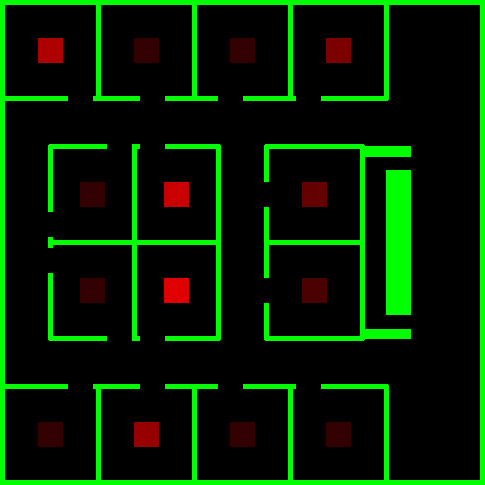
\includegraphics[width=\textwidth]{hospital}
        \centering
        \end{figure}

        \begin{table}[]
        \begin{tabular}{lll}
        Value & Atomic Proposition & Description                                                                                       \\
        225   & A                 & Start location of the agent. During operation, the agent will start at this location              \\
        200   & Z                 & End location. This is the last location the agent must travel to, in order to complete the task. \\
        175   & B                 & Atomic Proposition B                                                                               \\
        150   & C                 & Atomic Proposition C                                                                               \\
        ...   & ...               & ...                                                                                               \\
        75    & F                 & Atomic Proposition F
        \end{tabular}
        \end{table}

        \begin{figure}[h]
        \includegraphics[width=\textwidth]{hospital-cells}
        \centering
        \end{figure}

        \begin{figure}[h]
        \includegraphics[width=\textwidth]{hospital-cell-text}
        \centering
        \end{figure}

        \begin{figure}[h]
        \includegraphics[width=\textwidth]{hospital-cell-edges}
        \centering
        \end{figure}
    % Environment Processing and Risk

    \section{Task and Heuristic}
        The LTL task is given to the algorithm by a string or via a HOA file. In the case of the string, the Spot python library is used to convert the task equation into a buchii automata. In the case of the HOA file, a function parses though the file to create the following data structure. The automata is stored in a dictionary of dictionaries. The first key is the current node and the second key is the target node after the path jump. The value is the axiom that needs to be achieved to cause the path jump. For example to see what axiom is needed for a path jump from node 2 to node 5, `self.ltl\_stat\_dict[2][5]` can be used. This automata or graph can now be processed by the algorithm to construct our two heuristic models.

        The first heuristic being created is the node path length heuristic. The agent must get to an accepting state to complete the mission. By running the node distance part of the djikstra's algorithm, the shortest path length for each node can be calculated. An example of this is shown in Figure \Fig{}. At the starting node (node 1), the agent must take 3 hops to get to the accepting state. For nodes 3 and 4, the agent must take 2 hops. By attempting to minimize this number, the shortest path to the accepting state can be calculated. However, this method has its limitations. A sortest path in the LTL space may not be the shortest path in the environment space. To understand this issue, take the environment given in \Fig{}. The physical distance traveled when going from task A-B-C-Z is longer since it needs to double back when going from C to Z. However since the task does not force the ordering of B and C, another task path that can be taken is A-C-B-Z. In this case, the agent does not need to double back and also arrives at the accepting state of the LTL automata. To resolve this issue, we can use another heuristic: euclidean distance.

        % By utilizing Dijkstra's (DJK) algorithm to weight all the nodes in the LTL automaton graph, a very simple, albeit inefficient heuristic can be utilized. Since this automaton can be viewed as a graph, applying DJK's will lead to the shortest path on the LTL landscape graph. The graph search heuristic applies the DJK's algorithm to the graph above and weights each node by the distance to the closest accepting state. After applying this algorithm, the following heuristic is achieved. State 1 has a distance of 1 to the accepting state so it has a cost of 1. Both states 3 and 4 have a distance of 2 hops to the accepting state so the cost of these states is 2. By utilizing this cost map for the LTL task. Two separate algorithms can be run. A pathfinding algorithm on the LTL task graph and a pathfinding algorithm on the physical environment. Each jump in the LTL graph restarts the pathfinding algorithm on the physical environment. A large apparent flaw in this method is the issue of physical distance. If the B state on the physical environment is closer to the Z state than the C state is to the Z state, this issue is exacerbated. In other words. The path ABCZ would cause the agent to double back, causing delays. A simple example is shown below. By choosing path 2, an unnecessary double-backing of the agent can be avoided.

        The euclidean distance heuristic incorporates the information of the environment into the edges of the LTL graph. Each edge already has the axioms that need to be maximized to cause that path jump. However, now that edge also includes the euclidean distance as a weight of that edge. By utilizing this weight the distance to the accepting state can be approximated without having to run Dijkstra's on the entire graph. This cuts down on the time complexity immensely. An example of this can bee seen in \Fig{}. The path from A-B-C-Z can be approximated by the function ed(A, B) + ed(B, C) + ed(C, Z) which is much shorter than ed(A, B) + ed(B, C) + ed(C, Z). Some of the tasks that do not have a basis in the environment will not have this euclidean distance heuristic and will fall back to the previous, node distance heuristic.

        \begin{figure}[h]
            \includegraphics[width=\textwidth]{ltl-djk-graph}
            \centering
            \end{figure}

            \begin{figure}[h]
            \includegraphics[width=\textwidth]{ltl-djk-bad-ordering}
            \centering
            \end{figure}

            \begin{figure}[h]
            \includegraphics[width=\textwidth]{ltl-djk-good-ordering}
            \centering
        \end{figure}

    % Task and Heuristic

    \section{Partially Known Environments}
        One of the main applications of this algorithm is in the usage of it in a partially known or unknown environment. As the agent moves around it updated its internal data. Since each movement will uncover more of the environment, the old algorithm (product automata) would need to recompute the product automata and recalculate the trajectory the agent will travel. However, by utilizing the newer algorithm, the recomputation is unnecessary as the agent only computes the trajectory of its local (in both LTL space and environment space) neighborhood. An example of a partially known environment can be seen in \Fig{}. The environment is assumed to be a satellite imagery and does not contain

        A particular issue arises when attempting to use the previous algorithm in a dynamic or changing environment. At each step as more risk and more of the environment is uncovered, the product automata must be reconstructed at each step so the new information can be incorporated into the path that the agent must take. To remedy this issue, an alternative algorithm can be used: rather than reconstructing the product automata, the automata can be created on the fly. A separate set of issues arise, however, many of these issues can be fixed with the advent of additional benefits.

        One of the major benefits of this ad hoc method is the ability to incorporate live environmental data. Such as in the case of partially known environments and dynamic environments

    % Partially Known Environment

    \section{Partial Replanning}
        While the agent is moving around the environment, any new data it recives is only localized to the immediate of the agent. It then makes sense that the agent shouldn't compleately pathfind and can shortcut the A* algorithm. A circle is drawn with a radius two times the viewing distance and the intersection of the edge of this circle with the path planned is used to partial plan. Since the environment does not change outside the viewing distance, this is a good way to remove complexity in the A* algoirithm. This shortcut is only used if minimum changes to the environment is uncovered. If thershold for the change is triggered, a full replan is conducted.
    % Partial Replanning

    \section{Pathfinding}
        %
        At the start of the algorithm, the agent will preprocess the environment, this part includes lading the environment image from the disk, cellifying the environment, construction of the environment graph, and locating the LTL targets in the environment. The agent must also load the LTL graph either from the disk or using the Spot library, and the construct the ltl heuristic structures. Both of thede can be offloaded to a faster system even before the agent ventures into the environment. The details of preprocessing the environment is discussed in Section \ref{} and the preprocessing of the task is discussed in Section \ref{}.
        %
        Once the agent has preprocessed the environment and task, the agent can start moving through the environment. The algorithm is broken into two parts: path finding in the LTL domain and path finding in the physical domain. Similar to a nested loop, path finding in the LTL domain supersedes path finding in the physical domain. path finding in the physical domain is called after every jump in the LTL domain.
        %
        The steps for pathfinding in the LTL domain is shown in code block \ref{}. The agent steps through the task graph. At each node the agent requests the potential next stops it can take according to the graph. This list of target locations are passed to the heuristic functions (along with the heuristic structures) and the best target location is chosen. The agent then starts moving toward the chosen location. The environment movement occurs in the "inner loop" and is discussed in the following Section. Once the "inner loop" returns, the agent checks the current location to see which task was compleated and moved the task current node pointer to the appropriate next node. If the current location is not an task jump, the loop is rerun, since the inner loop may have returned to include a new task or of the sort. This cycle is repeated until the accepting state or the final state has been reached.
        %
        The steps for pathfinding in the environment domain is shown in code block \ref{}. each iteration of the loop represents movement from one cell to another. On each time step or movement, the agent observes the environment and updates its internal data structures with any new information obtained, and runs A* to the target cell recieved from the "outer loop". During this loop, the agent may recive a signal to change its task. In thise case the agent stops processing, updates its mission to include the new task and returns to the outter loop.
        %
        \begin{algorithm}
        \caption{Pathfinding Algorithm}\label{alg:cap}
        \begin{algorithmic}[1]
        \State \textbf{Input:} $\phi$
        \State \textbf{Output:}
        \Procedure{pathfind}{env, task}
            \State \Call{pathfind\_task}{accepting\_ltl\_state}
        \EndProcedure
        \State
        \Procedure{pathfind\_task}{accepting\_ltl\_state}
            \While{not in accepting ltl state}
                \State \Call{pathfind\_env}{target\_location}
            \EndWhile
        \EndProcedure
        \State
        \Procedure{pathfind\_env}{target\_location}
            \While{not at target location}
                \State \Call{move\_agent}{astar\_direction}
            \EndWhile
        \EndProcedure
        \end{algorithmic}
        \end{algorithm}

        Choosing which LTL target to travel to is carried out by the outside

        \begin{algorithm}
        \caption{Task Pathfinding Algorithm}\label{alg:cap}
        \begin{algorithmic}[1]

        \Function{pathfind\_task}{}
            \While{current LTL state is not an accepting state}
                \State get potential locations that would cause LTL path jump
                \State pick the optimal location based on heuristic
                \State \Call{pathfind\_env}{target\_location}
                \State move to next LTL state
            \EndWhile
        \EndFunction
        \end{algorithmic}
        \end{algorithm}

        \begin{algorithm}
        \caption{Environment Pathfinding Algorithm}\label{alg:cap}
        \begin{algorithmic}[1]

        \Function{pathfind\_task}{}
            \While{current location isnt the target location}
                \State update state using new environment information
                \State change target location if better option is available
                \If{the state changed greater than threshold}
                    \State \Call{astar}{}
                \Else
                    \State get partial astar target
                    \State \Call{partial\_astar}{}
                    \State combine partial astar path and original path
                \EndIf
                \State append current location to path
                \State \Call{move\_agent}{astar\_direction}
            \EndWhile
        \EndFunction
        \end{algorithmic}
        \end{algorithm}
    % Overview

% ALGORITHM


\chapter{EXAMPLES}
    The Algorithm described above is tested and applied to the following environments and missions. Each combination is tested and the results are recorded in the following section.
    % The problem targeted by this thesis is to create an efficient algorithm to construct a high level path for an agent to follow to complete an LTL based task while keeping the risk taken at a reasonable minimum in a changing or partially known environment.

    \section{Hospital}
        To include a trivial environment example, a simple hospital level is used. This allows the to showcase the features of this algorithm in its most basic form. The hospital is divided into two sections the reception (right) and back rooms. There are 14 rooms divided in four rows and each room has an opening to allow the agent to travel into the room to conduct its task. Since the hospital floor is usually known in civil blueprints, the agent will always know the full layout of the environment.

        % By using the basic task discussed in the preliminaries. We can see that the algorithm was able to create the proper path from A to C to B to Z.

        % \begin{figure}[h]
        % \includegraphics[width=\textwidth]{hospital-final-path}
        % \centering
        % \end{figure}

        % In a more complicated LTL task: $Fz \& (!z U c) \& (!z U e) \& G(d -> X(e \& !d)) \& (!e U d) \& G(b -> X(c \& !b)) \& (!c U b)$. This LTL formula has three important parts. Traversing to E must be preceded by D, traversing to C must be proceeded by B, and C and E must be completed before traveling to the final Z location. As you can see, the algorithm is able to compute a path without much of an issue.

        % \begin{figure}[h]
        % \includegraphics[width=\textwidth]{hospital-final-path-complex}
        % \centering
        % \end{figure}
    % Hospital

    \section{Military}
        To showcase the partially known environment, a military example is used. The environment is given to the agent as a satilight imagery. The image has a guassian blur applied to simulate the low resolution of satilight imagery. The green risk blobs can symbolize artilliry shell craters and other fallen debris.
        %
        As the agent traverses through the environment, the agent can update its own internal data structures with the information collected through its on-board sensors. This will update the risk from a partially known state to a fully known state. Partial replanning is also used in this example to test its efficacy. A task switch is also tested in this example to show the quick replanning of the agent with a new mission.
        %
        \begin{figure}[h]
        \includegraphics[width=\textwidth]{military-partial-ba}
        \centering
        \end{figure}

        \begin{figure}[h]
        \includegraphics[width=\textwidth]{military-final-path}
        \centering
        \end{figure}
    % Military

    \section{Space}
        For the last environment, a lunar surface is used. An actual lunar map is downloaded and used to create the risk landscape and the agent is then tasked with compleating two missions. This example serves the purpose of showing a more practical example with a real lunar environment.
        % @TODO INSERT IMAGE HERE
    % Space

    \section{Mission A}
        The first example mission for the agent is a simple A-spitBC-D task. The task offers a fork in the task that allows the agent to choose between paths. The mission serves the purpose of showcasing the euclidean distance heuristic. The agent will choose the path that minimizes the euclidean distance for the path. The LTL equation is written in equation \ref{}. and the resultant graph is shown in Figure \ref{}. Since the output of the Spot library contains many superflous edges, a cleaned up graph is pictured in Figure \ref{}. Please note that this is not the graph the agent will be working with. The algoirithm uses the full output of the library and this image serves the purpose of highlighting the two distinct paths the agent can take.
        % @TODO insert equation here
        % @TODO insert full graph here
        % @TODO insert pruned graph here
    % basic

    \section{Mission B}
        The second example mission is a more complicated A-splitBD-longBC-shortD-E task. The agent will be subject to the same fork as the previous simple example, however one fork will have a larger node distance than the other. This serves the purpose of testing the node distance heuristic. The agent will choose the shorter D path rather than the longer BC path. Note that the BC path may be taken in the case that BC path has a shorter euclidean distance than the D path. The euclidean distance heuristic takes precident over this node distance heuristic. Similarly to the simple example, equation \ref{} is the LTL equation for this task, Figure \ref{} shows the full graph, and Figure \ref{} shows a simplified graph.
    % complex

    \section{Mission C}
        The last example mission exemplifies a task switch scenario. A task is given to the agent and at some arbitrary time step, the agent recives a signal to switch tasks and the new task is loaded. Just like the previous two sections, equation \ref{} and \ref{} are the two LTL equations for this mission, Figure \ref{} and \ref{} shows the full graph, and Figure \ref{} and \ref{} shows a simplified graph.
    % basic --switch--> basic

% EXAMPLES


\chapter{RESULTS}
    % These are my results

    % environments/tasks (9)
    % Hospital A B C
    % Military A B C
    % Space A B C

    % Hospital with A and C missions in fully known environment
    % Military with B and C tasks in fully and partially known environment and partial replanning
    % Space with A and B tasks

    % independent vars (4)
    % - product automata
    % - fully known environment
    % - partially known environment
    % - partial replanning

    % dependent vars
    % - pathlength
    % - timing
% RESULTS


\chapter{DISCUSSION}
    % In the current age, attributing intelligence to computer systems is increasing in a accelerating rate. Algorithms like Large Language Models (LLN) have shown to exhibit human-like intelligence like humanity has never before. In a broad sense intelligence in navigation can be simplified into optimising a closed path between two points that satisfies certain conditions. In human evolution, theories have been made into how the hippocampal region of the brain first started out as a biological analogy to SLAM in robotics, this feature was generalized to include social tree mapping when humans evolved to communicate and live in larger social groups. Recent theories suggest that hippocampal activities may help in higher order problem solving and cognition. In many cases nature has paved way for engineering design. Similarly to how hippocamus place cells function to create a conscious and subconscious representation of where an agent is and planning future paths, this project gears to create a framework on how to better solve pathfinding problems. @TODO make this sound more relavent

    In previous works, these conditions were expanded into a bucci automate and then used graph theory to expand the set of all possible states the agent can be in. A major drawback of this process is that many states that the agent cannot access are also considered by the algorithm that is used. In this paper, by calculating the states live, while the agent is acting on the environment, the agent is able to update its state, pathfind in this space and avoid bad states in a faster and efficient manner.

    By considering two spaces. One for the abstract representation of the LTL states and another space of environmental states. The goal of the agent is to complete the LTL task by entering the accepting state of the automata. Thus, in a hierarchical view, the LTL task is superior to the environmental space. This allows the agent to mainly focus on completing and path finding through this higher-level abstract LTL space and rely on other path finding algorithms such as DJK, A* or partial A* for the environmental path finding.

    - intelligence systems / goal oriented bahavior and planning
    - mimic of these behaviors in automatic digital systems
    - use cases
    - interpretation of results
    - implecation of results
    - limitations
        - heuristic approach
        - new avenues in environment
        - performance over complexity/speed

    - future work

% DISCUSSION


\chapter{CONCLUSION}
    % In this project, the author presents a improved approach to pathfinding an environment with task contraints that allows a very large amount of modularity: adding tasks, removing tasks, incorporating risk and uncertainty in environment by utilizing a heuristic based multilayerd graph search algorithm. We remove the creation of a flattened product automata graph to introduce a "on the fly" calculation of the automata based off the neighborhood of nodes in both the task and environment space. To solve some challenges, some heuristics are introduced. We then utilized this algorithm to simulate an agent in 3 different environments with X different types of tasks. The reults were compared to other variations to the algorithm and pros and cons of each were discussed. Other heuristics can be added that can be beneficial in other contexts. In the case of a multi agent system, the heuristic can be updated with the actual physical path for other agents to use (embeddeing rich metrics into the graph) and Artificial Intelligence can be added to convert english worded tasks into LTL tasks. Many of these improvments are left for future work.
    %
    In this project, the author introduces a novel and refined approach to the problem of path finding in environments characterized by task constraints, emphasizing its inherent capacity for extensive modularity. This modularity is manifest in the incorporation of new tasks, removal of existing tasks, and the effective integration of risk and uncertainty within the environment and mission. These objectives are achieved through the deployment of a heuristic-based multilayered graph search algorithm. A noteworthy departure from convention is the elimination of the conventional practice involving the creation of a flattened product automata graph. Instead, the research advocates for the dynamic, on-the-fly computation of the automata, derived from the localized network of nodes residing in both the task and environmental spaces. To address the manifold challenges posed by the problem at hand, a suite of heuristic strategies is introduced to augment the path finding process.
    %
    Subsequently, this algorithm is used to simulate an agent's traversal within three distinct environmental contexts, each under a diverse array of missions. The resultant outcomes are meticulously scrutinized in comparative fashion alongside the original product automata approach and other variations of the novel approach, thereby affording a comprehensive examination of the merits and demerits associated with each.
    %
    Furthermore, it is posited that the algorithm's utility can be further extended through the incorporation of additional heuristics, tailored to specific contextual exigencies. In the context of multi-agent systems, the heuristic framework can be dynamically updated to encompass the actual physical paths traced by coexisting agents, thereby enhancing the graph with more detailed and contextually relevant metrics. Additionally, a novel facet of artificial intelligence is introduced, serving the purpose of translating human-readable task descriptions into Linear Temporal Logic (LTL) representations. It is important to acknowledge that several of these proposed enhancements remain subjects for future research and development, thus underlining the ongoing nature of this scholarly pursuit.
% CONCLUSION


\fbmatterchapterformat

\bibliographystyle{ieeetr}
\bibliography{references_db}


\newpage{}\uncctocformat{chapter}{0pt}{350pt}{\appendixname~\thecontentslabel:~}
\renewcommand{\chaptertitlename}{APPENDIX}
%
% The default setting for appendices excludes sections, subsections, etc. from
% the TABLE OF CONTENTS.
% If you want these in the TABLE OF CONTENTS, increase the number in the line below:
% 1 - Appendices, Sections / 2 - Appendices, Sections, Subsections / 3 - etc
%
\addtocontents{toc}{\protect\setcounter{tocdepth}{0}}

\appendix

    \section{CLI PARAMETERS}

        The appendices should be used for whatever material you or your advisory
        committee believes should be included, but would not be appropriate
        in the text of the thesis or dissertation. Such materials can include:
        \begin{enumerate}
            \item the original data obtained in the thesis or dissertation research,
            including computer programs and printouts, surveys, or correspondence;
            \item detailed descriptions of procedures, which go beyond the general outline
            of methods and approaches presented in the text;
            \item a particularly extensive review of the literature and other information
            that may be useful to future scholars who may wish to delve more deeply
            into the research topic.
        \end{enumerate}
    % CLI PARAMETERS

    \section{Section in appendix}
    This is a section in the appendix.
% appendix

\end{document}
